\documentclass[paper=A4, DIV=10, parskip=half]{scrartcl}

% Udacity Links
% -------------

% Project Review Rubric:
% https://review.udacity.com/#!/rubrics/2345/view

% Examples:
% https://github.com/udacity/machine-learning/blob/master/projects/capstone/report-example-1.pdf
% https://github.com/udacity/machine-learning/blob/master/projects/capstone/report-example-3.pdf

% Link to Capstone Proposal Review
% https://review.udacity.com/#!/reviews/2779272

% Packages
% --------

\RequirePackage{hyperref}
\RequirePackage{xcolor}
\hypersetup{%
  colorlinks=false,% hyperlinks will be black
  linkbordercolor=darkgray,% hyperlink borders will be red
  pdfborderstyle={/S/U/W 1}% border style will be underline of width 1pt
}
\RequirePackage{graphicx}
\RequirePackage[english]{babel}
\RequirePackage{listings}
\RequirePackage{amsmath}
\RequirePackage{amsfonts}
\RequirePackage{float}

% Document Head
% -------------

\title{Dog Breed Identification}
\subtitle{Project Report}
\author{Grzegorz Lippe}
\date{\today}

\begin{document}

\maketitle

\lstset{% general command to set parameter(s)
  language=Python,
  numbers=left,
  keywordstyle=\color{blue},
  commentstyle=\color{violet},
  numberstyle=\tiny,
  breaklines=true,
  basicstyle=\footnotesize\ttfamily, % typewriter type for strings
  showstringspaces=false} % no special string spaces

%\begin{abstract}
  
\section*{Definition}

\subsection*{Project Overview}

In this project the knowledge and usage of Convolutional Neural Networks (CNN)
is demonstrated for the Udacity reviewer team. Within this project a CNN with
the ability to detect dog breeds with an accuracy of more than 10\,\% is created
from scratch. Afterwards a pre-trained
VGG16\footnote{\href{https://pytorch.org/vision/0.8/models.html}{Pytorch Models}}
\footnote{\href{https://arxiv.org/abs/1409.1556}{Very Deep Convolutional
Networks for Large-Scale Image Recognition}} is adapted to perform the same task
with an accuracy of $>$60\,\%.

Besides a neural net for dog breed detection, also an existing
OpenCV\footnote{\href{https://opencv.org/}{Open Computer Vision}} neural net for
face recognition is adapted. The algorithm provides a bounding box for each face
it found within a picture.

Both algorithms, the OpenCV face recognition and the VGG16 dog breed detection
are combined into an demo app, that can take an arbitrary picture and return a
statement of a most likely dog breed. If a picture of a human is provided, the
app should identify the human, but still provide a statement of a most similar
looking dog breed.

% Student provides a high-level overview of the project in layman’s terms. Background
% information such as the problem domain, the project origin, and related data sets or
% input data is given. 

%\end{abstract}

%\newpage
%\tableofcontents
%\newpage


\subsection*{Problem Statement}

Given that the human face recognition is a takeover OpenCV network, the problem
solved is the identification of a dog breed with the help of a convolutional
neural network.

% The problem which needs to be solved is clearly defined. A strategy for solving the
% problem, including discussion of the expected solution, has been made.

\subsection*{Metrics}

For the evaluation the labelled data is used. For example the accuracy of the face
detection algorithm can be measured by feeding it with (previously labelled) images of
humans: 

$$ Score = \frac{\textrm{Humans detected}}{\textrm{Images presented}}$$

A slightly modified algorithm is used to evaluate the dog detecting model. The dog
detector provides a breed identification on top, so in the first step the upper term can
be used to judge the accuracy of the dog detection. Additionally the quality of the breed
identification is measured as follows:

$$ Score = \sum_{breeds}{\frac{\textrm{correct breed identified}}{\textrm{breed provided}}} $$


% Metrics used to measure the performance of a model or result are clearly defined.
% Metrics are justified based on the characteristics of the problem.

\section*{Analysis}

\subsection*{Data Exploration}

The data consists of two different sets, provided by Udacity and are described as follows:

\begin{description}
  \item[\href{https://s3-us-west-1.amazonaws.com/udacity-aind/dog-project/dogImages.zip}{dog dataset}]
  The dog data set is already divided into three different datasets (folders)
  for test, training and validation. Each folder contains sub directories of the specific
  formating \texttt{DDD.breed\_name}, where \texttt{DDD} represents a 3 digit number,
  followed by the breed name after a dot. Each subfolder contains a hand full of images of
  the specific breed.
  
  Overall there are 133 different dog breeds, and 835 images provided for validation, 6680
  images for training and 836 images for testing. The images within the training dataset
  are unbalanced, the amount of images per breed varies from 26 for the Norwegian Buhund
  and the Xoloitzcuintli to 77 for the Alaskan Malamute. So some breeds are represented
  roughly 3 times more often.
  
  The dog images contain a singular dog each, mostly of the whole dog, sometimes only of
  the snout, but they are not equally sized, they vary from 5 kB up to 5 MB. Their aspect
  ratios cover all ranges between portrait, landscape and quadratic.
  
  \item[\href{https://s3-us-west-1.amazonaws.com/udacity-aind/dog-project/lfw.zip}{human dataset}]
  The human dataset consists of 13233 images of 5749 persons, which are stored in a
  separate directory named after each  celebrity. The images of the people are already
  cropped and centred around their face and all of the same size of 250x250, but
  the backgrounds vary. Sometimes there are additional people in the background.
\end{description}

% If a dataset is present, features and calculated statistics relevant to the problem have
% been reported and discussed, along with a sampling of the data. In lieu of a dataset, a
% thorough description of the input space or input data has been made. Abnormalities or
% characteristics of the data or input that need to be addressed have been identified.

\subsection*{Exploratory Visualization}

\subsubsection*{Human Dataset}

Here is a random sample of the human images dataset:

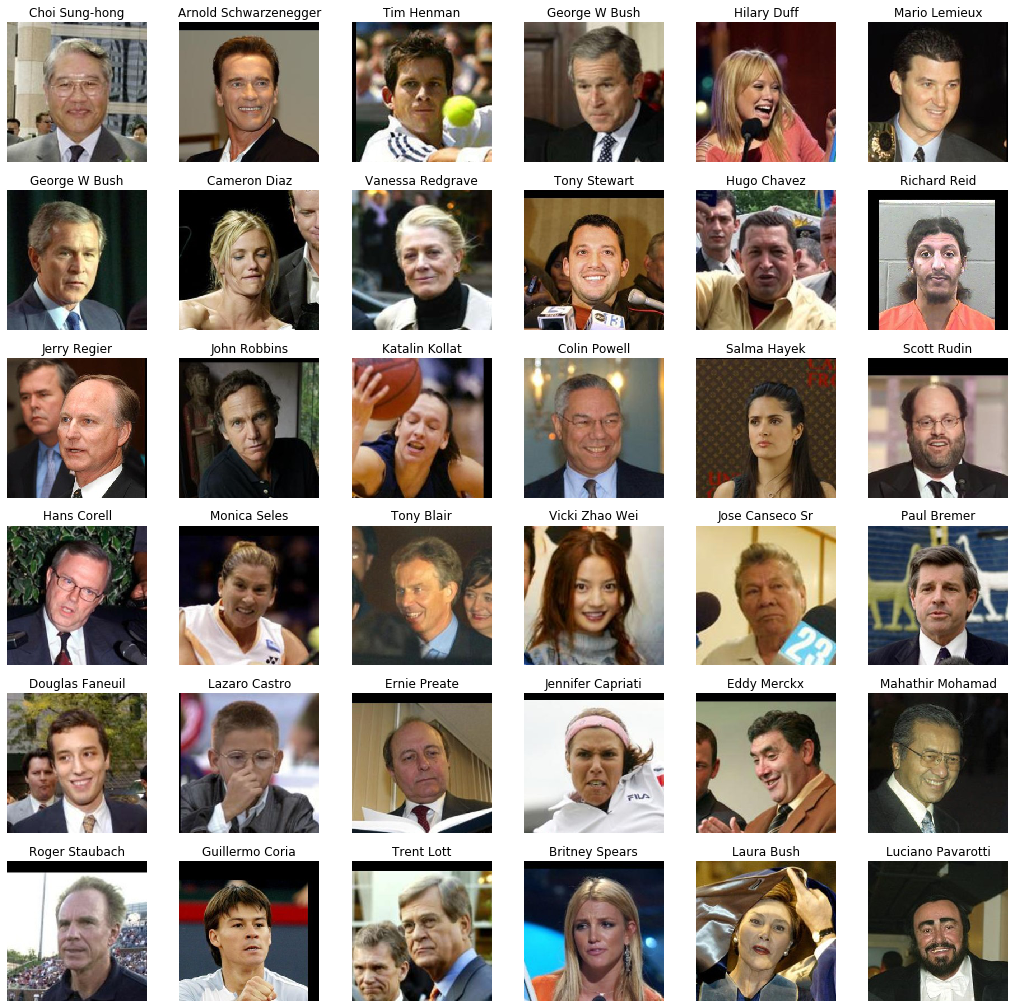
\includegraphics[width=\textwidth]{images/human_sample.png}

Its worth noticing, that George Bush appeared two times in this randoms sample
of 36 images out of 13233, so this is a hint for an unbalanced dataset. A
further investigation of the dataset confirms the suspicion, the following bar
plot, figure \ref{human_balance} in the appendix, shows the amount of pictures
of the top 25.

George Bush, Collin Powell and Tony Blair alone are represented in 910 Images or
roughly seven percent of the dataset. On the other hand 4069 celebrities of the
5749 persons are represented by only one image.
%, see figure \ref{human_tail_sample}:

% \begin{figure}[h]
%   \centering
%   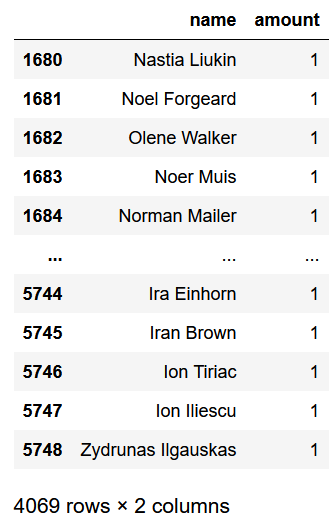
\includegraphics[height=6cm]{images/human_tail_sample.png}
%   \caption{4069 celebrities are represented in the human dataset with only one picture each}
%   \label{human_tail_sample}
% \end{figure}

If the problem at hand would be the training of a face recognition algorithm
this unbalanced dataset would be a problem, but within this project it is only
used for sample data sets to test the demonstrator app with later.

\subsubsection*{Dog Dataset}

Here is a random sample of the dog images dataset:\\
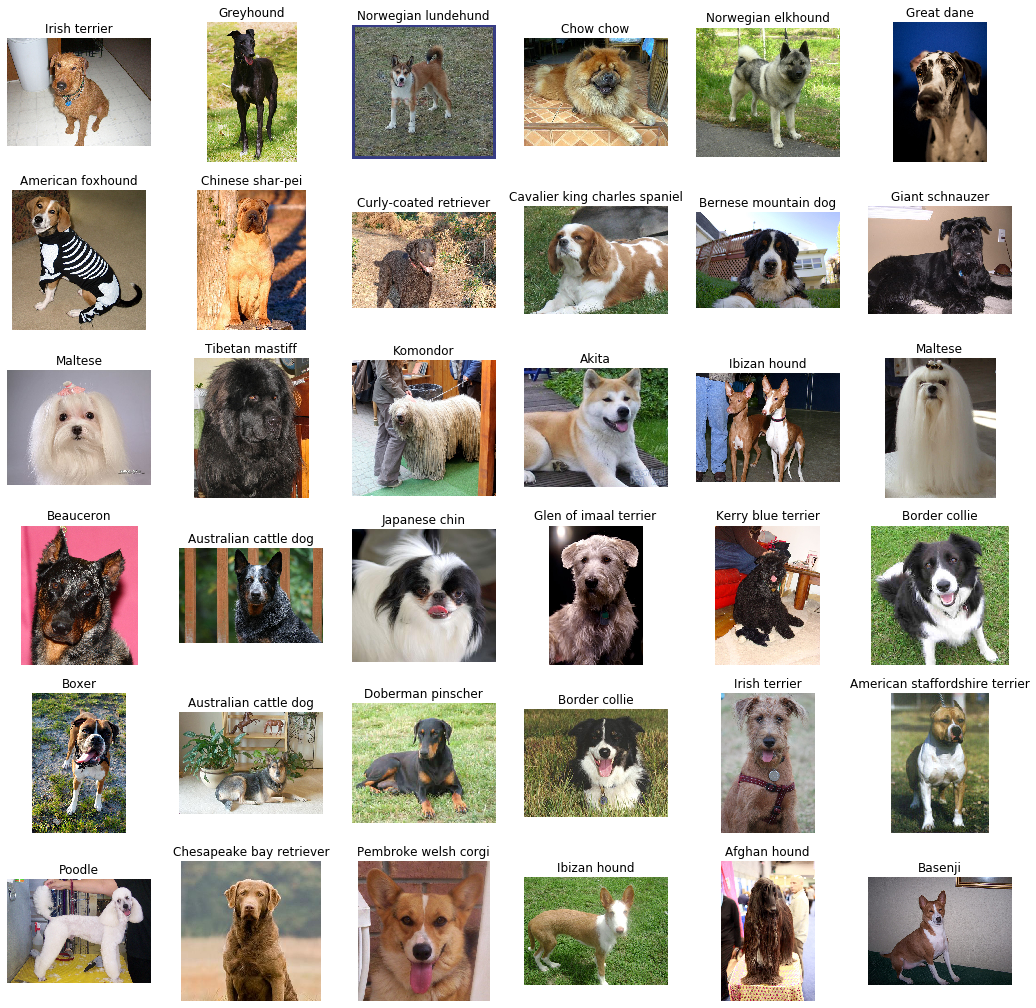
\includegraphics[width=\textwidth]{images/dog_sample.png}

At a first glance everything is fine, there are images of dogs, sometimes whole
dogs and sometimes their snouts only. Therefore a more thorough investigation is
performed.

The following table shows the amount of breeds (count) for each subset: "train",
"test" and "valid". The mean value shows how many images are present in average
in every breed: 50.

\begin{center}
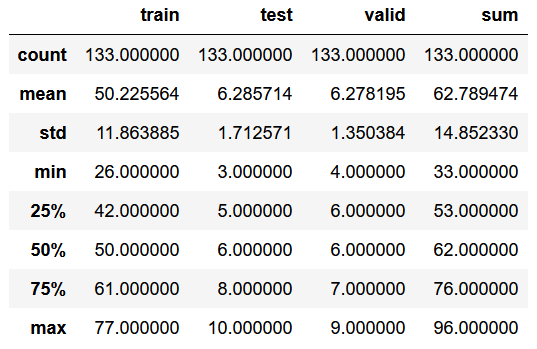
\includegraphics[width=7cm]{images/dog_deviation.png}
\end{center}

Also it states, that there are at least 26 images for each
breed in the training set and 77 at best. A more visual representation about the
balance of the data set is provided in the appendix within this document in the
bar plot \ref{dog_train_balance}.

Additionally also the sizes and aspect ratios of the images matter. These were
investigated by extracting these information out of each file and storing them
in a Pandas\footnote{\href{pandas.pydata.org/}{Panel Data}} DataFrame for
further investigation. 

The following figure \ref{dog_image_sizes} shows a logarithmic histogram of the
file sizes of the dog images. Most images are roundabout 100 kB in size,
starting at 4 kB but leading up to 10 MB.

\begin{figure}[H]
  \centering
  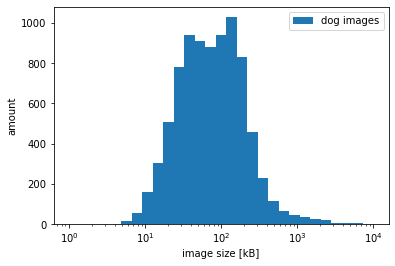
\includegraphics[height=5cm]{images/dog_image_sizes.png}
  \caption{Histogram of the dog image sizes [kB, logarithmic]}
  \label{dog_image_sizes}
\end{figure}

The top 5 image sizes were inspected visually and the biggest image in the
dataset is some image of two people at a dog show. This image, see figure
\ref{dog_extreme} is not suitable for training and therefore discarded from the
dataset.

In the same manner the top and bottom five aspect ratios where investigated. The
image with the "highest" Aspect ratio is a montage of two Lhasa Apso dogs, which
is fine to use in the test data set.

\begin{figure}
  \centering
  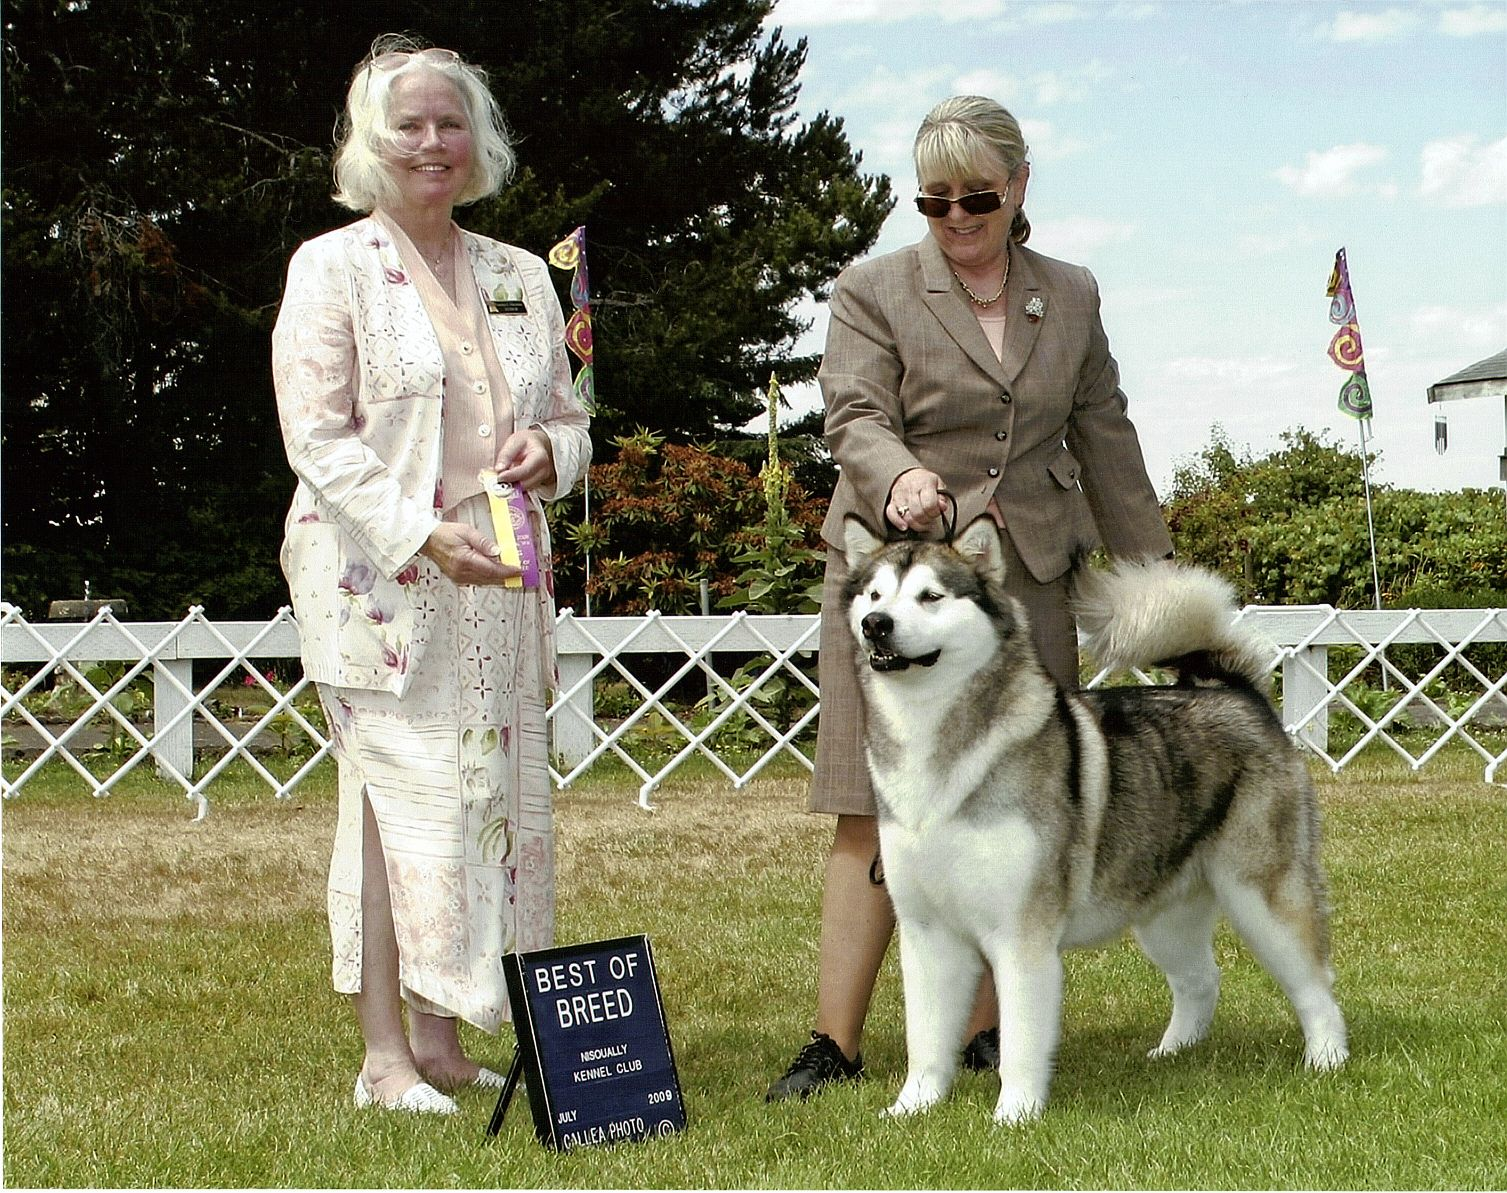
\includegraphics[width=5cm]{images/Alaskan_malamute_00366.jpg}
  \,
  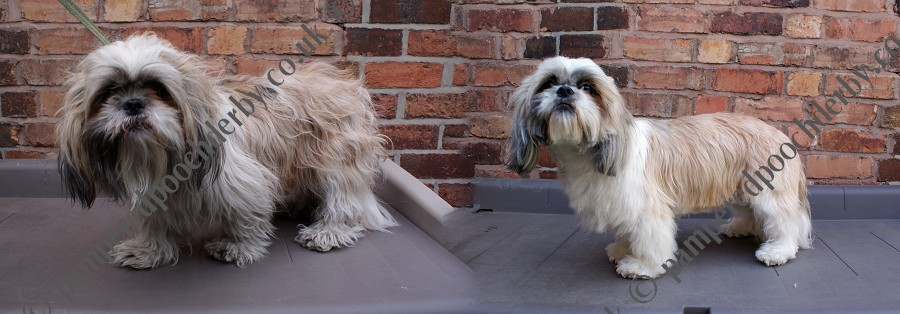
\includegraphics[width=6cm]{images/Lhasa_apso_06668.jpg}
  \caption{The maximum sized image and the maximum aspect ration image of the dog dataset}
  \label{dog_extreme}
\end{figure}

% A visualization has been provided that summarizes or extracts a relevant characteristic
% or feature about the dataset or input data with thorough discussion. Visual cues are
% clearly defined.

\subsection*{Algorithms and Techniques}

The problem of the dog breed identification will be solved using a convolutional
neural network. These networks are especially good on solving the tasks of image
recognition, within a 2-dimensional space. 

Whereas classical neural networks depend on a flat input vector and usually
fully connect the different layers, in a convolutional network many different
subsets of images are analysed with the help of a so called kernel. The kernel
can be thought of as a kind of filter, which extracts the information that
pixels have in relation to one another, like for example a horizontal line. This
extracted information than is passed on to another layer and can be abstracted
even more.

\begin{figure}[H]
  \centering
  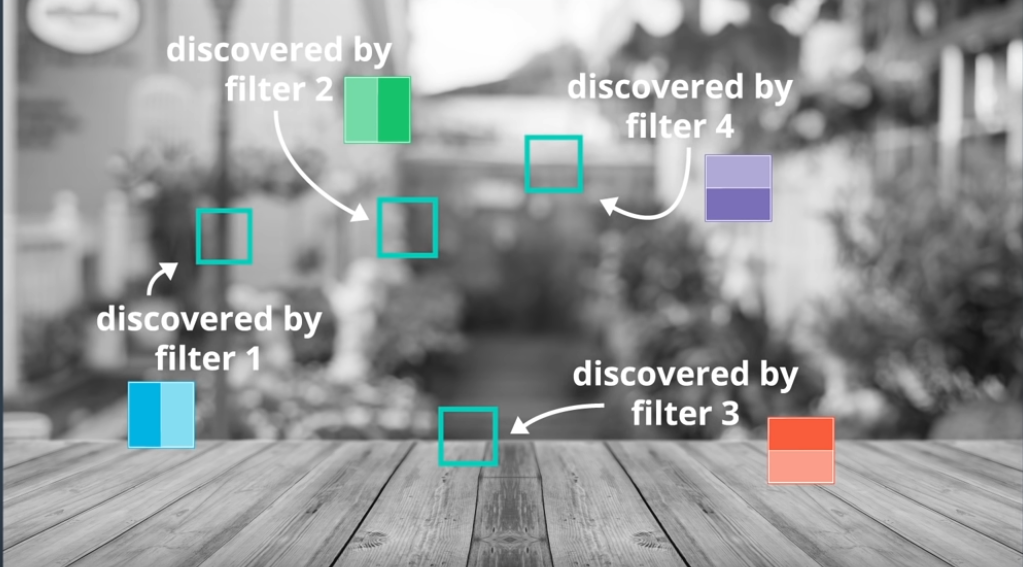
\includegraphics[width=7cm]{images/different_kernels.png}
\caption{A scheme of how different kernels detect different features, source:
\href{https://youtu.be/RnM1D-XI--8?t=181}{Udacity}}
  \label{different_kernels}
\end{figure}

Figure \ref{different_kernels} shows an Udacity example of how four different
kernels detect four different kinds of features in an image:
\begin{itemize}
  \item horizontal lines from dark to light
  \item horizontal lines from light to dark
  \item vertical lines from dark to light and
  \item vertical lines from light to dark.
\end{itemize}

The whole training of a CNN is the optimization of the weights in the
different kernels of the neural net. So the CNN learns to extract different
features of images within the training task.

% Algorithms and techniques used in the project are thoroughly discussed and properly
% justified based on the characteristics of the problem.

\subsection*{Benchmark}

As a benchmark I will use a naive predictor. The dataset is slightly unbalanced so
assuming that there are 133 different dog breeds, some of the occurring up to three times
more than others, the naive approach should guess the correct breed $(b)$ with
$p_{b}=\frac{k_{b}}{3\cdot133}\,,\:k_{b}=\left[1\ldots3\right]$, or less than 1\%. The
implemented model shall get at least 10\%.

% Student clearly defines a benchmark result or threshold for comparing performances of
% solutions obtained.

\section*{Methodology}

\subsection*{Data Preprocessing}

The images are preprocessed and augmented in three different kinds, for the
testing, the training and the validation data set.

\begin{lstlisting}[caption=Image Transformation, label=image_transformation]
# documentation values:
# https://pytorch.org/docs/stable/torchvision/transforms.html
normalize = transforms.Normalize(mean=[0.485, 0.456, 0.406],  
                                 std=[0.229, 0.224, 0.225])   

training_transform = transforms.Compose([transforms.RandomResizedCrop(256),
                                     transforms.RandomHorizontalFlip(),
                                     transforms.ToTensor(),
                                     normalize])

validation_transform = transforms.Compose([transforms.Resize(300),
                                     transforms.CenterCrop(256),
                                     transforms.ToTensor(),
                                     normalize])

test_transform = transforms.Compose([transforms.Resize(size=(256,256)),
                                     transforms.ToTensor(),
                                     normalize])
\end{lstlisting}

Listing \ref{image_transformation} shows all image preprocessing steps performed
for the training of the CNN. All in common for the testing, validation and
training data set is a normalization and a transformation into a
\lstinline{torch.transforms.ToTensor()} data type.

The normalization takes place with documented values and changes the
representation of the integer RGB values $\underline{n} \in \mathbb{N}^3, [0
\ldots 255]$ to normalized float values $\underline{q} \in \mathbb{Q}^3, \left[0.0
\ldots 1.0\right]$. Two dimensions for the image, the third for the colour.

The test dataset gets an additional resize to a quadratic shape $256^2$. If the
image was portrait or landscape before it now is squeezed, but that doesn't
matter for the recognition task. I chose 256, because it is a power of 2.

The validation dataset undergoes a different transformation. It is first resized
and then cropped to the center, because the validation images all contain the
dog in the center of the image.

The training dataset a different kind of resize, the
\lstinline{RandomResizedCrop}. This causes the image to be cropped at a random
position of the in put image. Therefore the training data may or may not
contain an whole dog or just a part of a dog. This leads to a harder training
with better results and prevents over fitting. For the same reason the training
dataset also is preprocessed with a random horizontal flip.

% All preprocessing steps have been clearly documented. Abnormalities or characteristics
% of the data or input that needed to be addressed have been corrected. If no data
% preprocessing is necessary, it has been clearly justified.

\subsection*{Implementation}

\subsubsection*{Transfer Learning with a pre trained Network}

The adaption of the pre trained VGG16 neural network is thoroughly described in
the Udacity Lesson "Transfer Learning" within the extra curricular
material\footnote{\href{https://classroom.udacity.com/nanodegrees/nd009-ent/parts/a73e944a-fdd9-4469-9c67-a618aab59b18/modules/7862c5aa-2097-4dfa-9776-cbfe245d7b83/lessons/a559990d-e214-4c5d-a424-437f6299383e/concepts/bd6c99ac-2c4f-4a80-9ae4-adb4403666c2}{Transfer
Learning Lesson}} for the "Machine Learning Engineer Nano Degree". Essentially
the VGG16 network was trained on the \href{http://www.image-net.org/}{image-net}
data base with 14 million images and can extract 1000 classes within the
image-net database. These 1000 labels are defined by the last fully connected
layer of the CNN, see figure \ref{vgg16arch}.

\begin{figure}[H]
  \centering
  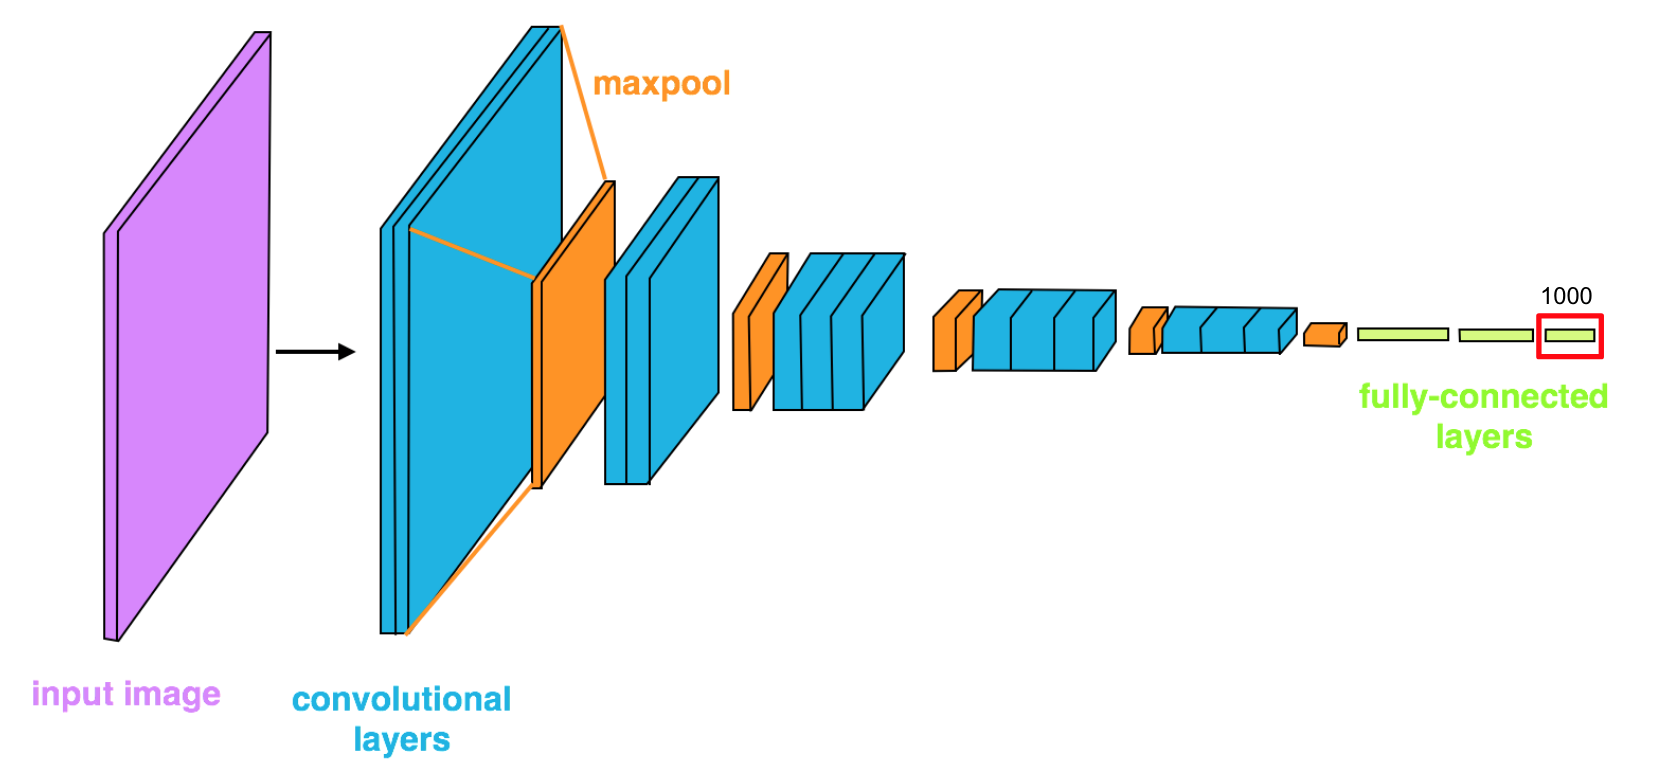
\includegraphics[width=10cm]{images/vgg_16_architecture.png}
  \caption{VGG-16 Architecture, Source: Udacity}
  \label{vgg16arch}
\end{figure}

The benefit of such a highly trained network is, that all the image recognition
filters, which are there to recognise a vast amount of different geometrical
artifacts like: horizontal lines, vertical lines, circles etc. are already
there. Moreover the subsequent pooling and convolutional layers are also trained
to identify more complex shapes like: wheels, aeroplanes, or fur.

Therefore the neural net can be adapted and retrained, by only changing the last
layer, which defines the 1000 labels of the VGG16. The following listing
\ref{orig_class} shows the classifier of the VGG, which correspondent to the
three green boxes in figure \ref{vgg16arch}:

\begin{lstlisting}[caption=Original VGG16 Classifier, label=orig_class]
Sequential(
  (0): Linear(in_features=25088, out_features=4096, bias=True)
  (1): ReLU(inplace=True)
  (2): Dropout(p=0.5, inplace=False)
  (3): Linear(in_features=4096, out_features=4096, bias=True)
  (4): ReLU(inplace=True)
  (5): Dropout(p=0.5, inplace=False)
  (6): Linear(in_features=4096, out_features=1000, bias=True)
)
\end{lstlisting}

There are three fully connected linear layers, the last one providing 1000 nodes
for 1000 image classes. The dog breed data set contains 133 breeds, so the
following three lines of code reconfigure the model \ref{reconf}.

\begin{lstlisting}[caption=Adapting VGG16 Classifier, label=reconf]
  # Freeze training for all "features" layers
  for param in model_transfer.features.parameters():
      param.requires_grad = False
  
  model_transfer.classifier[6] =  nn.Linear(4096, 133) # from the flower exercise I knew there are 4096 input nodes in the second to last layer
\end{lstlisting}

The fist two lines of code tell the model to not adapt (require gradients)
within the training process. With that option the already existing and capable
neural net will be preserved during training. The last line changes tha last
fully connected layer to provide 133 exit nodes. These are trainable and will be
adapted within the training process. 

After that the model is provided with a loss function
(\lstinline{torch.nn.CrossEntropyLoss}) and a optimization function
(\lstinline{torch.optim.SGD}) it is trained on the Udacity dog image test set.

\subsubsection*{Creating a CNN from Scratch}

There are some additional questions which have to be solved when creating a CNN
from scratch, beginning with the required image size. The image size for the VGG
is 224x224 by definition so this question did not come up.

I chose a image size of 256x256. Since it is a little bit larger than the VGG I
will not loose to much detail. By setting the size to a power of 2 $(2^8)$ I
would not have had troubles with halfing the image sizes during the pooling
layers.

Second question to solve is how many convolutional and pooling layers shall the
custom neural net have? The next listing \ref{orig_features} shows the first six
layers of the VGG feature architecture from figure \ref{vgg16arch}:

\begin{lstlisting}[caption=Original VGG16 Features, label=orig_features]
Sequential(
  (0): Conv2d(3, 64, kernel_size=(3, 3), stride=(1, 1), padding=(1, 1))
  (1): ReLU(inplace=True)
  (2): Conv2d(64, 64, kernel_size=(3, 3), stride=(1, 1), padding=(1, 1))
  (3): ReLU(inplace=True)
  (4): MaxPool2d(kernel_size=2, stride=2, padding=0, dilation=1, ceil_mode=False)
  (5): Conv2d(64, 128, kernel_size=(3, 3), stride=(1, 1), padding=(1, 1))
  (6): ReLU(inplace=True)
  (7): Conv2d(128, 128, kernel_size=(3, 3), stride=(1, 1), padding=(1, 1))
  (8): ReLU(inplace=True)
  (9): MaxPool2d(kernel_size=2, stride=2, padding=0, dilation=1, ceil_mode=False)
...
)
\end{lstlisting}

Taking a closer look at the initial stack:

\begin{enumerate}
\item A convolutional layer receiving 3 features (RGB values of the input image)
and providing 64 output layers.
\item The second layer is also a convolutional one, providing the same amount of
features 64.
\item a max pooling layer, halfing the image size to 112.
\item a convolutional layer expanding the amount of features from 64 to 128.
\item a second convolution layer.
\item another max pooling layer, halfing the image size to 56.
\end{enumerate}

it can bee seen, that the amount of features roughly doubles after each pooling
and the kernel size is 3 for all convolutional layers. I decided to adapt that
approach and started with only one convolutional layer with 16 features.This was
already able to identify 3\,\% of the dog images correctly, which is more it
could have achieved by randomly guessing. 

Afterwards the amount of features was doubled with each convolutionl layer and
after each layer the dimensions where reduced by a factor of 2. The neural net
with 3 convolutional layers (listing \ref{custom_cnn}) was able to identify
10\,\% of the dog breed after training for 15 Epochs.

\begin{lstlisting}[caption=Custom Design CNN, label=custom_cnn]
class Net(nn.Module):
  def __init__(self):
    super(Net, self).__init__()
    # convolutional layer (sees 256x256x3 image tensor)
    self.conv1 = nn.Conv2d(3, 16, 3, padding=1)

    # convolutional layer (sees 128x128x3 tensor)
    self.conv2 = nn.Conv2d(16, 32, 3, padding=1)

    # convolutional layer (sees 64x64x3 tensor)
    self.conv3 = nn.Conv2d(32, 64, 3, padding=1)
...
\end{lstlisting}

It is worthwhile to notice that the custom CNN has 64 features, but can identify
133 dog breeds. That is, because each possible combination of theses features
is a different point in $\mathbb{Q}^{64\times64}$.

% The process for which metrics, algorithms, and techniques were implemented with the
% given datasets or input data has been thoroughly documented. Complications that occurred
% during the coding process are discussed.

\subsection*{Refinement}

\begin{itemize}
\item The dog images dataset could be refined using the human face detection algorithm
to clean it from unwanted people in the dataset.
\item Different augmentations, for example rotation of the images would lead to
a better trained model, but also higher CPU/GPU usage.
\item A weight initialization of the CNN would speed up the training effect and
increase the prediction accuracy.
\end{itemize}

% The process of improving upon the algorithms and techniques used is clearly documented.
% Both the initial and final solutions are reported, along with intermediate solutions, if
% necessary.

\section*{Results}

\subsection*{Model Evaluation and Validation}

\begin{itemize}
  \item The CNN implemented from Scratch provided a test accuracy of : 10\,\%
  (88/836)
  \item The Transfer Learning VGG16 model provides a test accuracy of 84\,\% (705/836)
\end{itemize}

% The final model’s qualities—such as parameters—are evaluated in detail. Some type of
% analysis is used to validate the robustness of the model’s solution.

\subsection*{Justification}

The Both models performed way better than I expected, I am a little proud that I
was able to learn to create and adapt these models.


% The final results are compared to the benchmark result or threshold with some type of
% statistical analysis. Justification is made as to whether the final model and solution
% is significant enough to have adequately solved the problem.

\newpage
\section*{Appendix}

\begin{figure}[H]
  \centering
  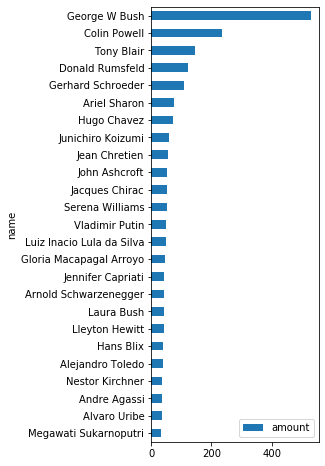
\includegraphics[height=11cm]{images/human_balance.png}
  \caption{Top 25 celebrities represented in the human dataset}
  \label{human_balance}
\end{figure}

\begin{figure}
  \centering
  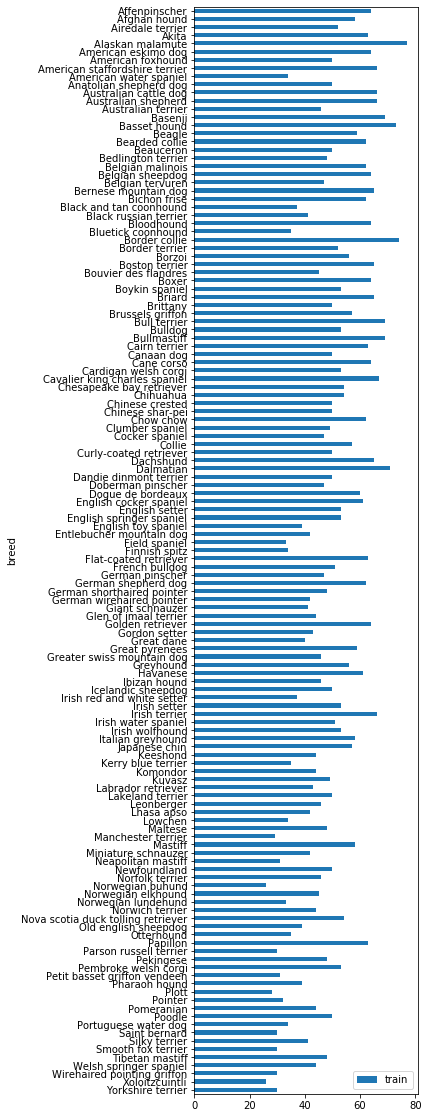
\includegraphics[height=0.95\textheight]{images/dog_train_balance.png}
  \caption{Balance of the Dog Breeds within the dog data set}
  \label{dog_train_balance}
\end{figure}


\end{document}
